\documentclass[tikz,crop]{standalone}

\usetikzlibrary{
  positioning,
  arrows,
  fit
}

\begin{document}
  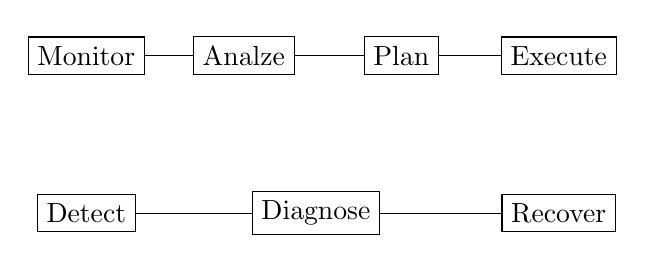
\begin{tikzpicture}[
    auto,node distance=2cm,
    stepNode/.style={draw,outer sep=0pt},
  ]
    % MAPE-K loop
    \node[stepNode] (monitor) {Monitor};
    \node[stepNode, right of=monitor] (analyze) {Analze};
    \node[stepNode, right of=analyze] (plan) {Plan};
    \node[stepNode, right of=plan] (execute) {Execute};
    
    \draw[-,black] (monitor) -- (analyze)  -- (plan) -- (execute);
    
    % self-healing loop
    \node[stepNode, below of=monitor] (detect) {Detect};
    \node[fit={(analyze) (plan)}] (anchor) {};
    \node[stepNode, below of=anchor] (diagnose) {Diagnose};
    \node[stepNode, below of=execute] (recover) {Recover};
    
    \draw[-,black] (detect) -- (diagnose) -- (recover);
  \end{tikzpicture}
\end{document}